\documentclass[11pt]{article}

\usepackage{outlines}
\usepackage{graphicx}
\usepackage[T1]{fontenc}
\usepackage{subcaption}
\usepackage[margin=1in]{geometry}

\usepackage{geometry}
\usepackage[square,sort,comma,numbers,super]{natbib}
\usepackage{pdflscape}
\usepackage{hyperref}
\usepackage{afterpage}

\usepackage[utf8]{inputenc}
\usepackage{xcolor}
\definecolor{textblue}{rgb}{.2,.2,.7}
\definecolor{textred}{rgb}{0.54,0,0}
\definecolor{textgreen}{rgb}{0,0.43,0}

\usepackage{listings}

\lstset{language=Java, 
numbers=left, 
numberstyle=\tiny, 
stepnumber=1,
numbersep=5pt, 
tabsize=4,
basicstyle=\ttfamily,
keywordstyle=\color{textblue},
commentstyle=\color{textred},   
stringstyle=\color{textgreen},
frame=none,                    
columns=fullflexible,
keepspaces=true,
xleftmargin=\parindent,
showstringspaces=false}

\graphicspath{ {./images/} }

\setlength{\parindent}{0pt}

% pt = project title; shorthand
\newcommand{\pt}{Multi-User Poker Game}
\newcommand{\pn}{Rekop}

\title{Interim Report: \pt}
\author{James Scully}

\setcounter{tocdepth}{4}

\setcounter{secnumdepth}{5}


\begin{document}

{\fontfamily{cmss}\selectfont}



\newcommand{\cardheight}{6em}

\newcommand{\tenclubs}{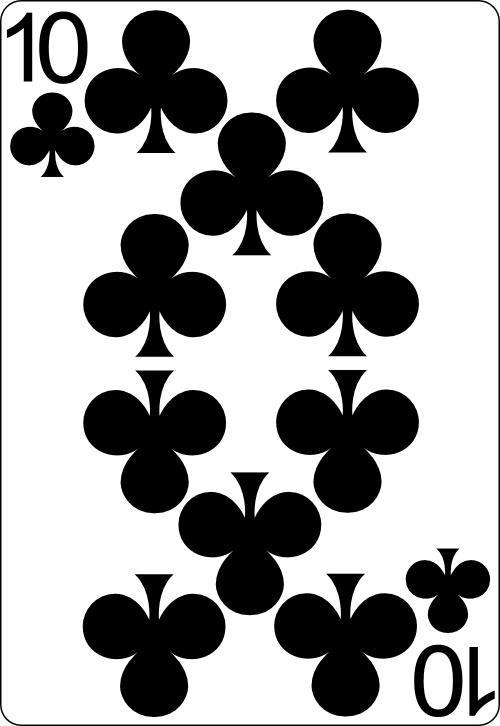
\includegraphics[height=\cardheight]{cards/10_of_clubs.png}}
\newcommand{\tendiamonds}{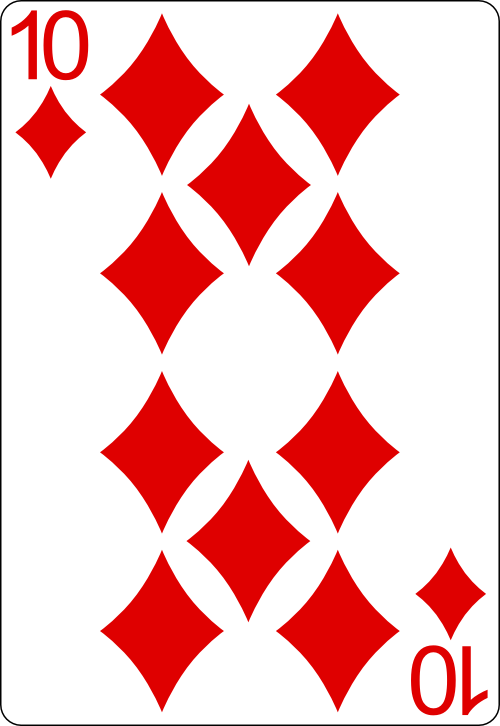
\includegraphics[height=\cardheight]{cards/10_of_diamonds.png}}
\newcommand{\tenhearts}{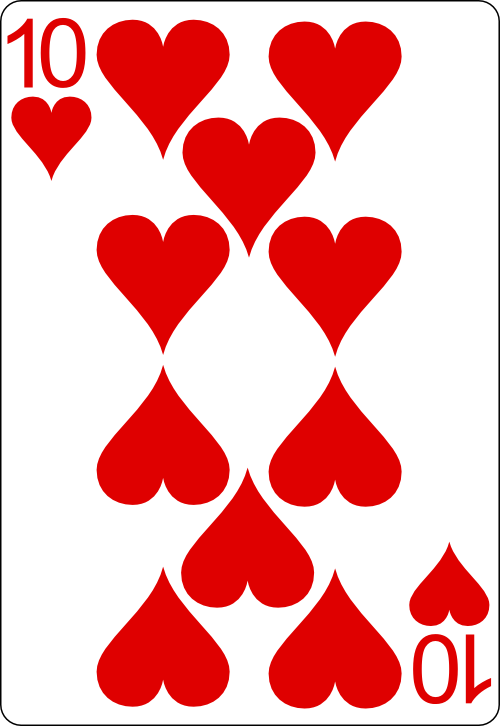
\includegraphics[height=\cardheight]{cards/10_of_hearts.png}}
\newcommand{\tenspades}{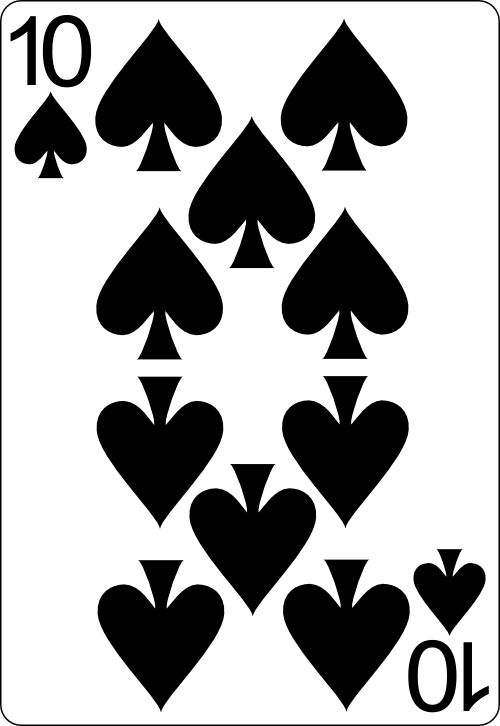
\includegraphics[height=\cardheight]{cards/10_of_spades.png}}
\newcommand{\twoclubs}{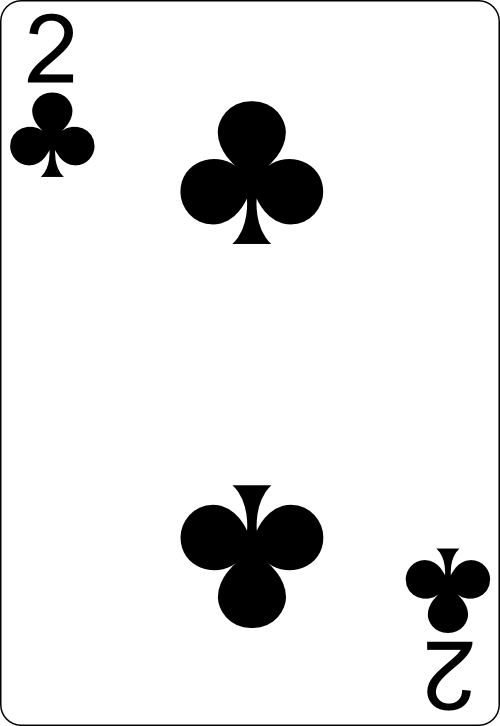
\includegraphics[height=\cardheight]{cards/2_of_clubs.png}}
\newcommand{\twodiamonds}{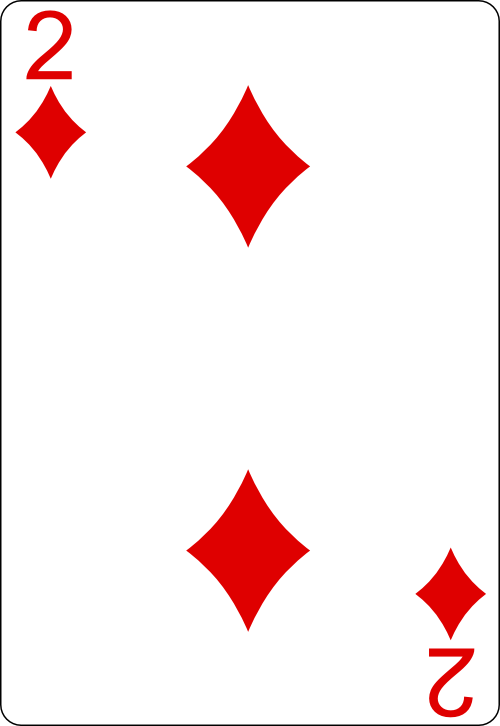
\includegraphics[height=\cardheight]{cards/2_of_diamonds.png}}
\newcommand{\twohearts}{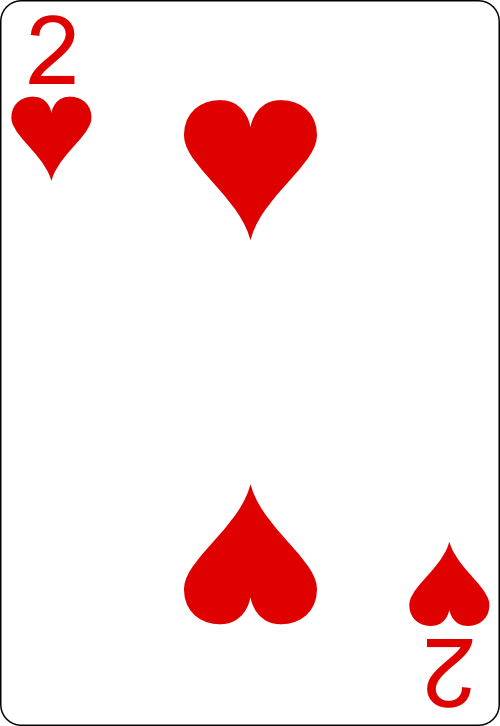
\includegraphics[height=\cardheight]{cards/2_of_hearts.png}}
\newcommand{\twospades}{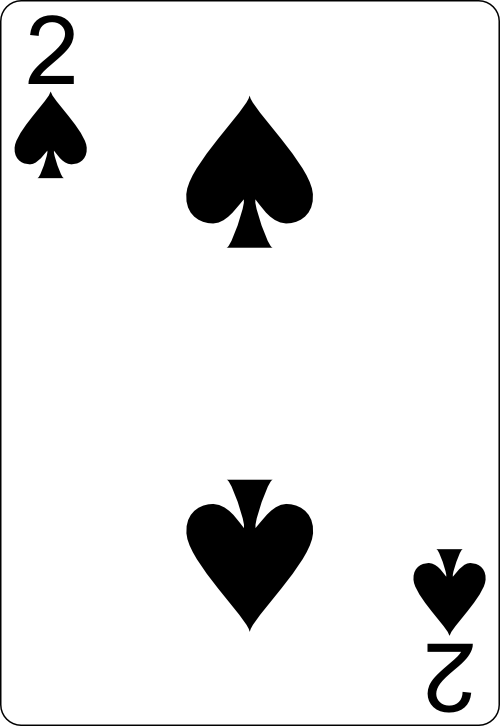
\includegraphics[height=\cardheight]{cards/2_of_spades.png}}
\newcommand{\threeclubs}{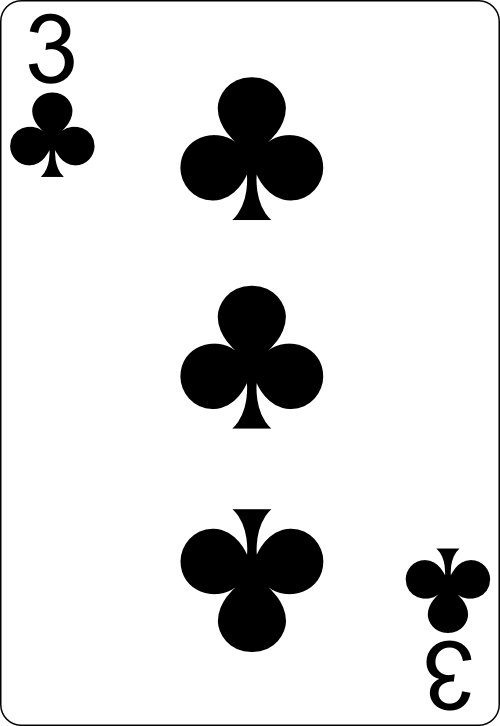
\includegraphics[height=\cardheight]{cards/3_of_clubs.png}}
\newcommand{\threediamonds}{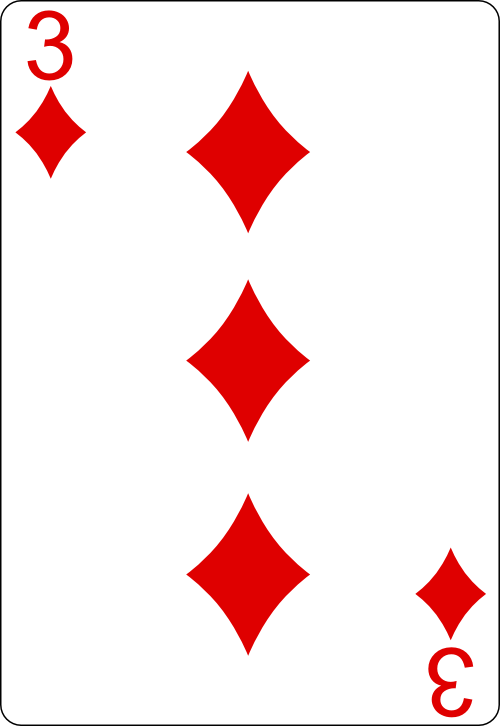
\includegraphics[height=\cardheight]{cards/3_of_diamonds.png}}
\newcommand{\threehearts}{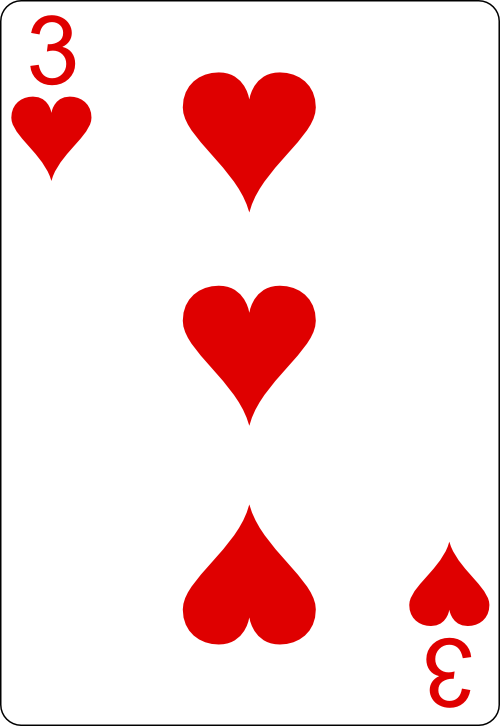
\includegraphics[height=\cardheight]{cards/3_of_hearts.png}}
\newcommand{\threespades}{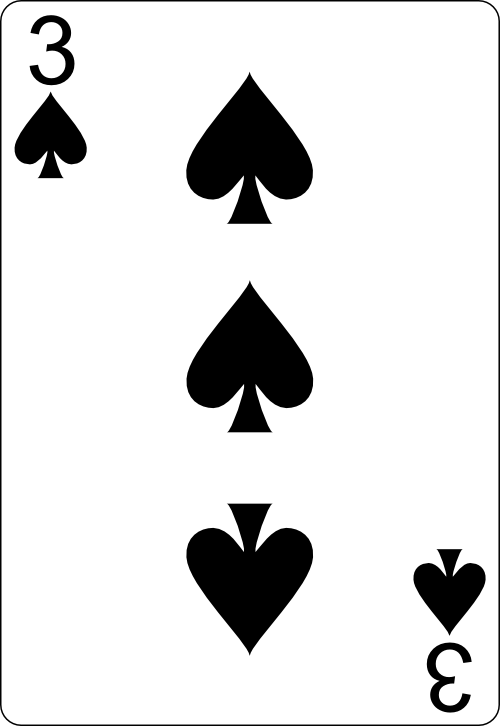
\includegraphics[height=\cardheight]{cards/3_of_spades.png}}
\newcommand{\fourclubs}{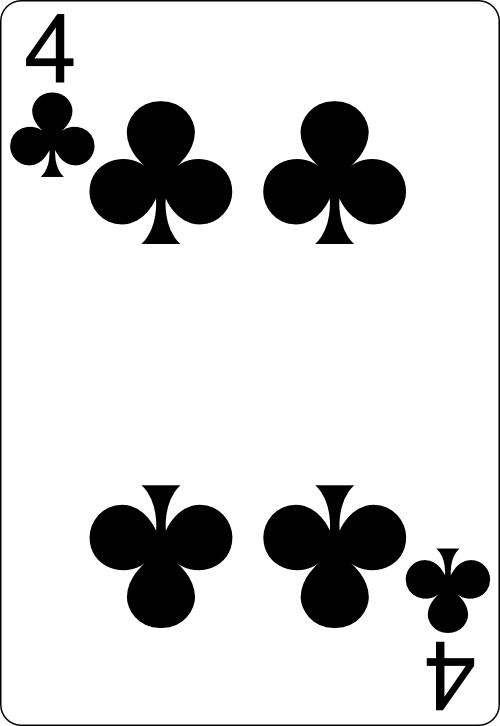
\includegraphics[height=\cardheight]{cards/4_of_clubs.png}}
\newcommand{\fourdiamonds}{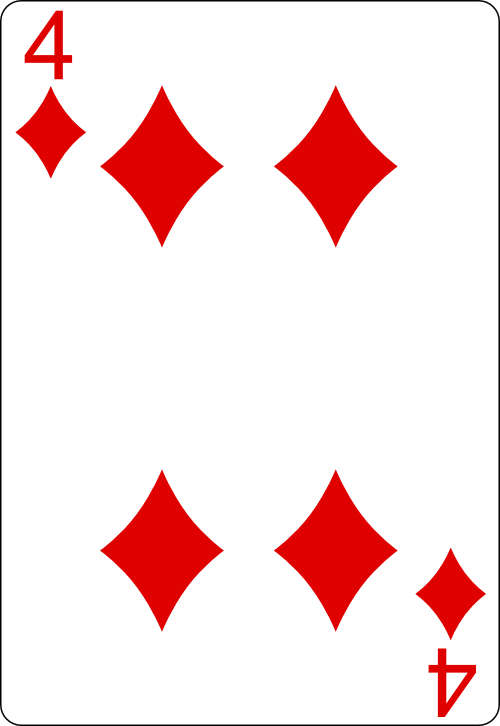
\includegraphics[height=\cardheight]{cards/4_of_diamonds.png}}
\newcommand{\fourhearts}{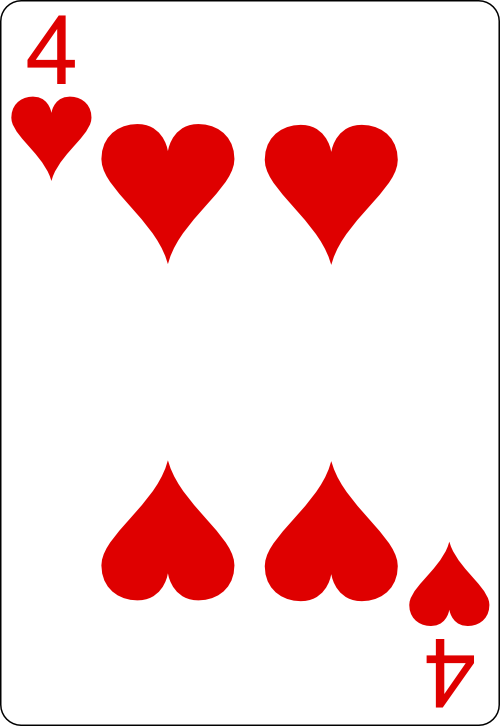
\includegraphics[height=\cardheight]{cards/4_of_hearts.png}}
\newcommand{\fourspades}{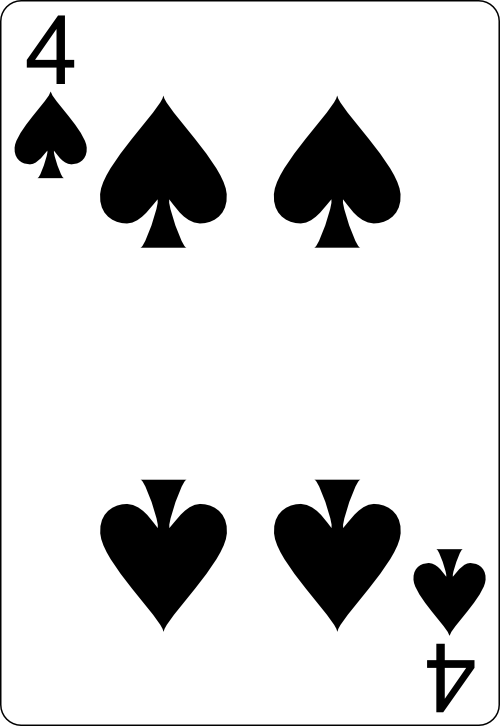
\includegraphics[height=\cardheight]{cards/4_of_spades.png}}
\newcommand{\fiveclubs}{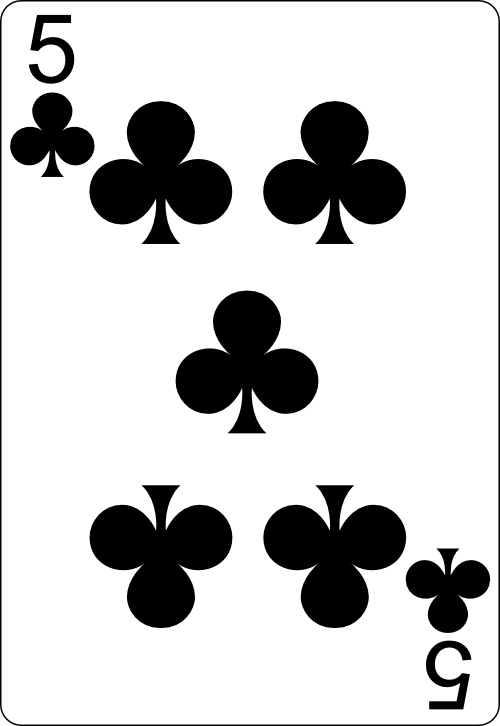
\includegraphics[height=\cardheight]{cards/5_of_clubs.png}}
\newcommand{\fivediamonds}{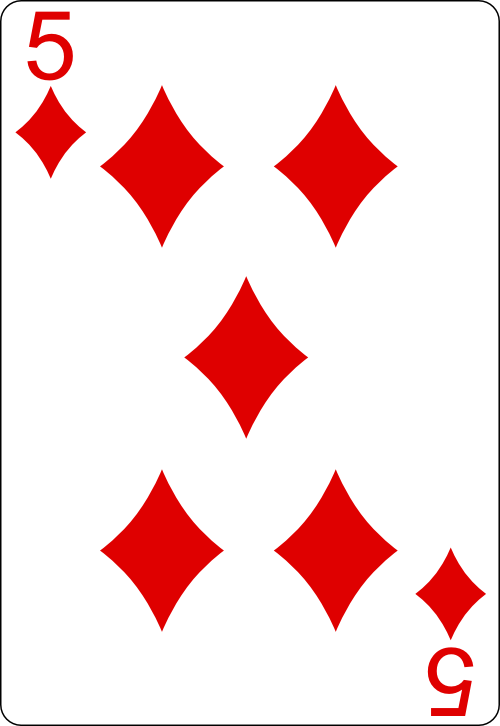
\includegraphics[height=\cardheight]{cards/5_of_diamonds.png}}
\newcommand{\fivehearts}{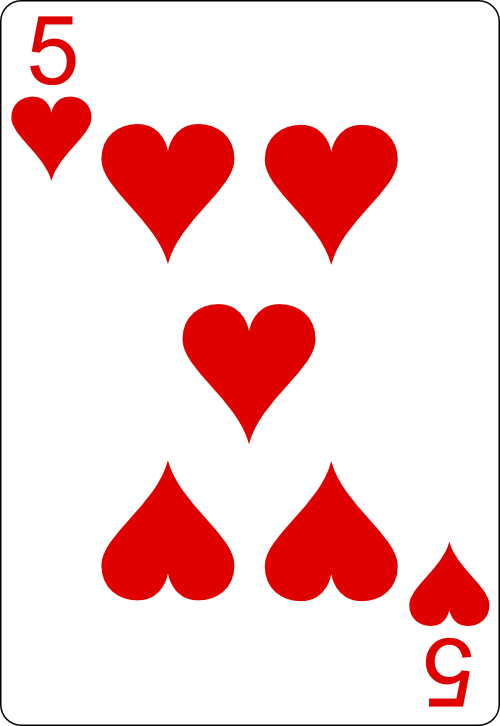
\includegraphics[height=\cardheight]{cards/5_of_hearts.png}}
\newcommand{\fivespades}{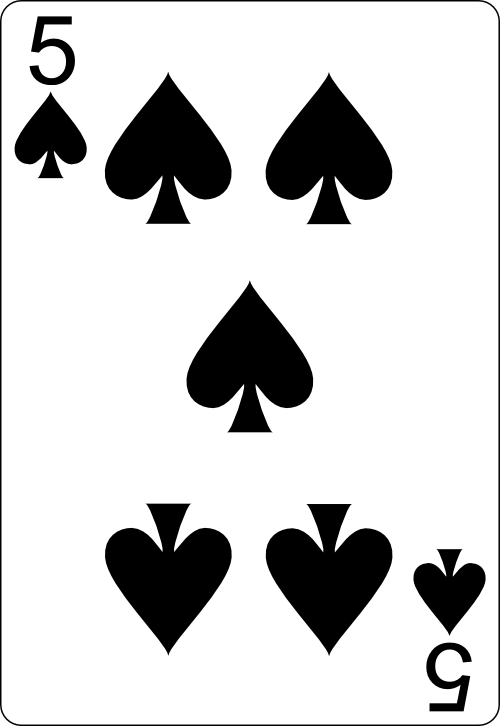
\includegraphics[height=\cardheight]{cards/5_of_spades.png}}
\newcommand{\sixclubs}{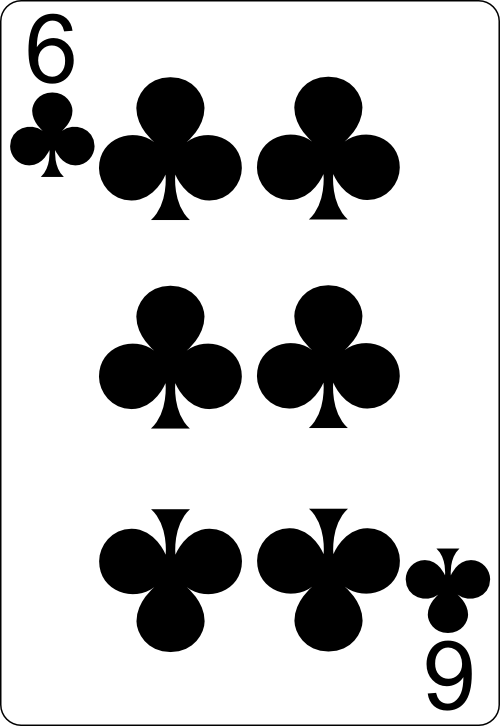
\includegraphics[height=\cardheight]{cards/6_of_clubs.png}}
\newcommand{\sixdiamonds}{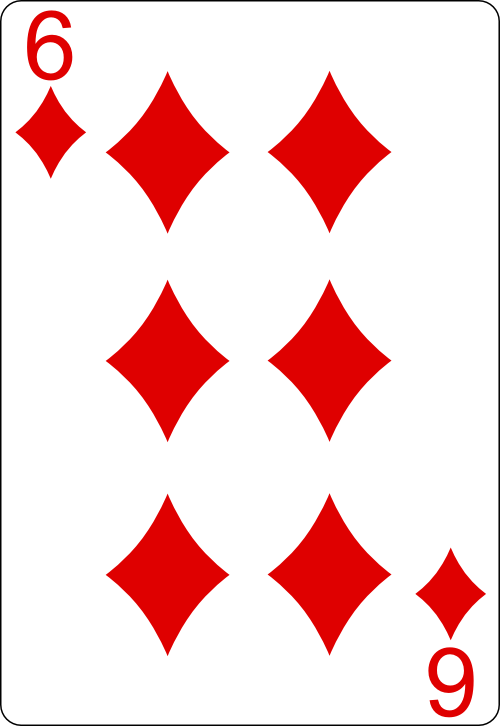
\includegraphics[height=\cardheight]{cards/6_of_diamonds.png}}
\newcommand{\sixhearts}{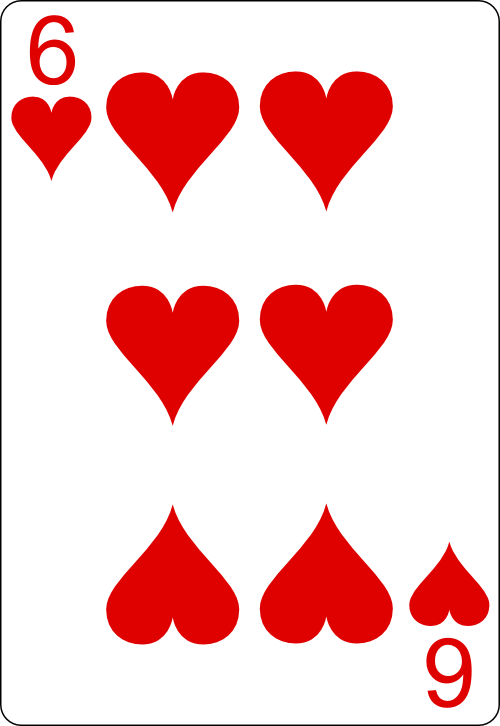
\includegraphics[height=\cardheight]{cards/6_of_hearts.png}}
\newcommand{\sixspades}{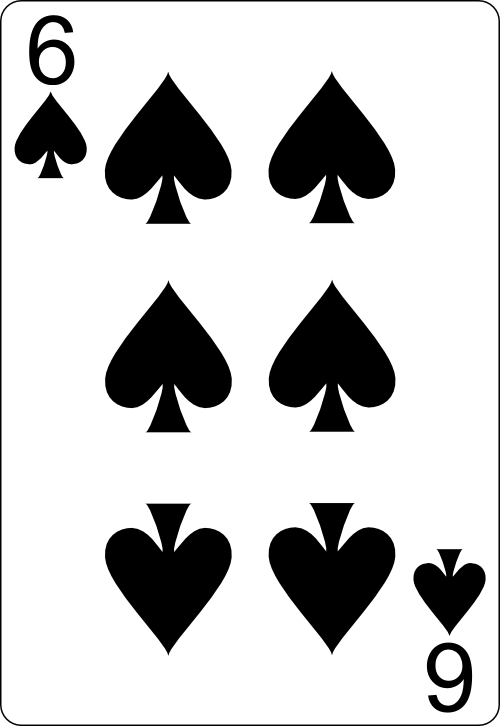
\includegraphics[height=\cardheight]{cards/6_of_spades.png}}
\newcommand{\sevenclubs}{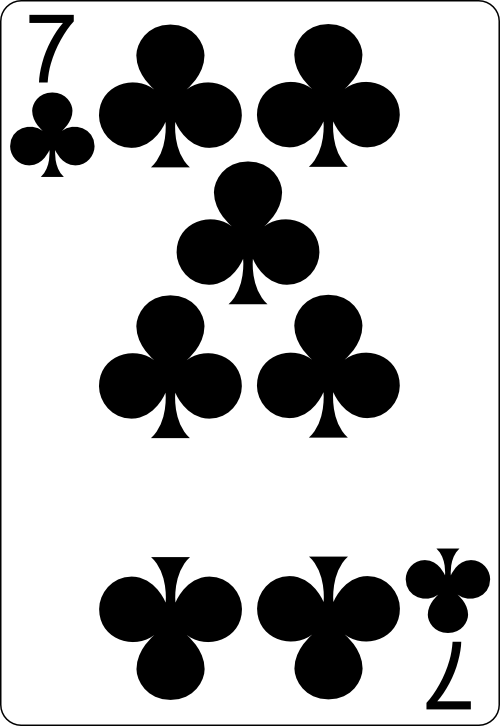
\includegraphics[height=\cardheight]{cards/7_of_clubs.png}}
\newcommand{\sevendiamonds}{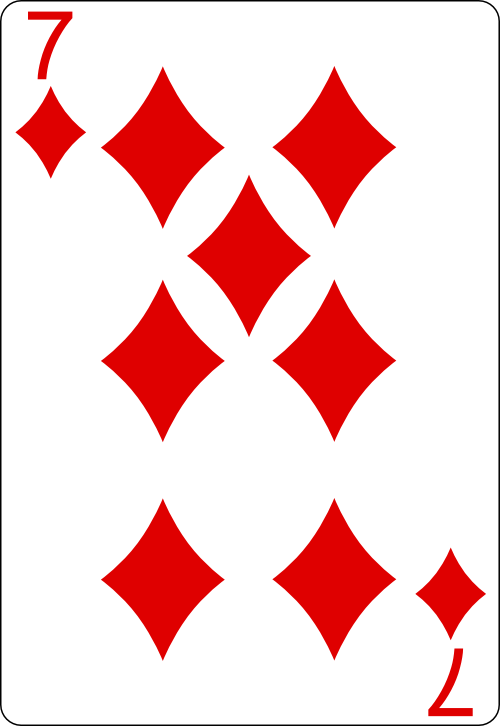
\includegraphics[height=\cardheight]{cards/7_of_diamonds.png}}
\newcommand{\sevenhearts}{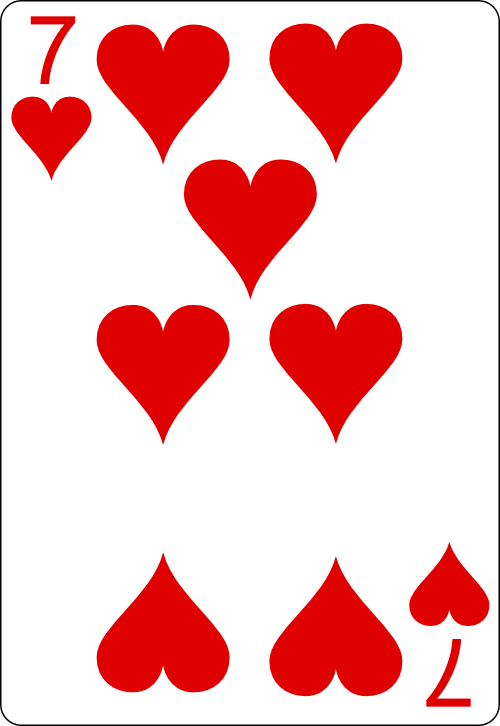
\includegraphics[height=\cardheight]{cards/7_of_hearts.png}}
\newcommand{\sevenspades}{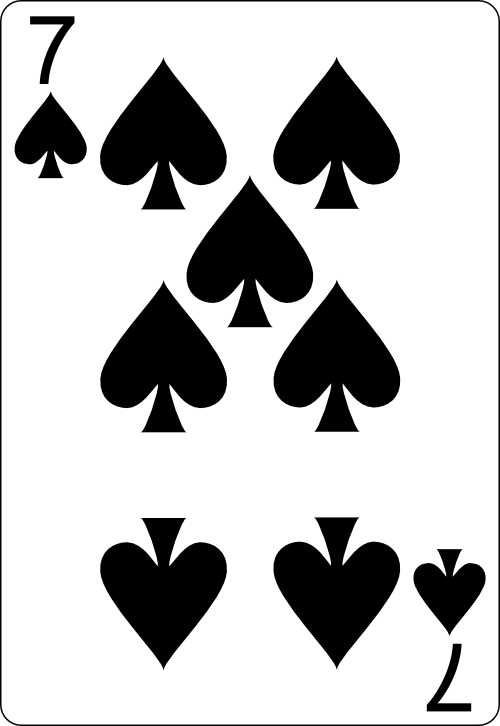
\includegraphics[height=\cardheight]{cards/7_of_spades.png}}
\newcommand{\eightclubs}{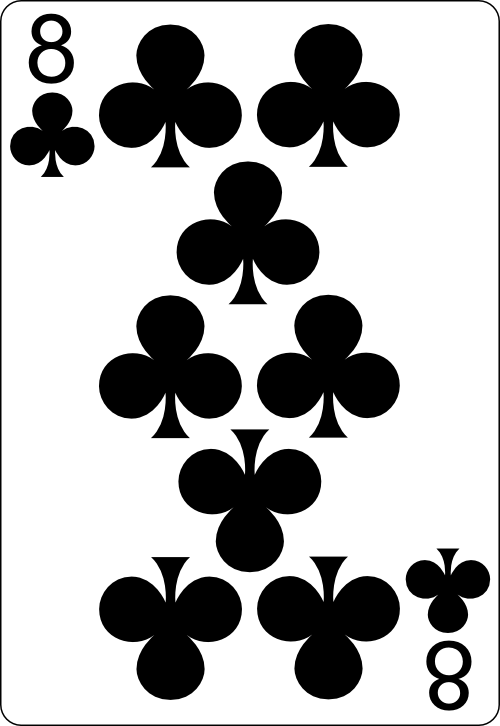
\includegraphics[height=\cardheight]{cards/8_of_clubs.png}}
\newcommand{\eightdiamonds}{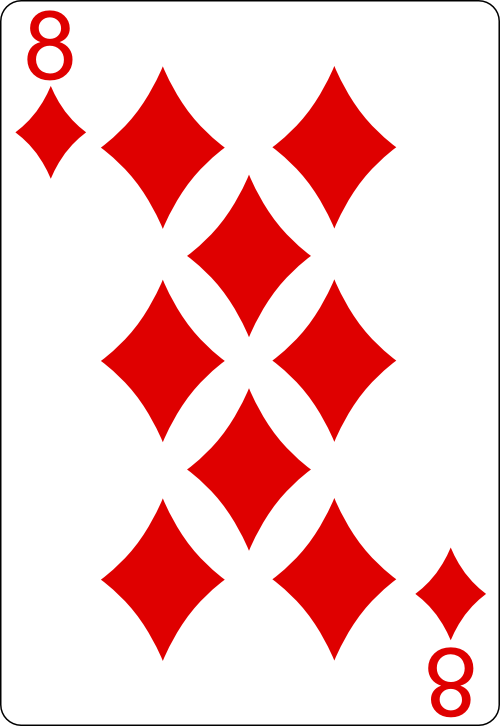
\includegraphics[height=\cardheight]{cards/8_of_diamonds.png}}
\newcommand{\eighthearts}{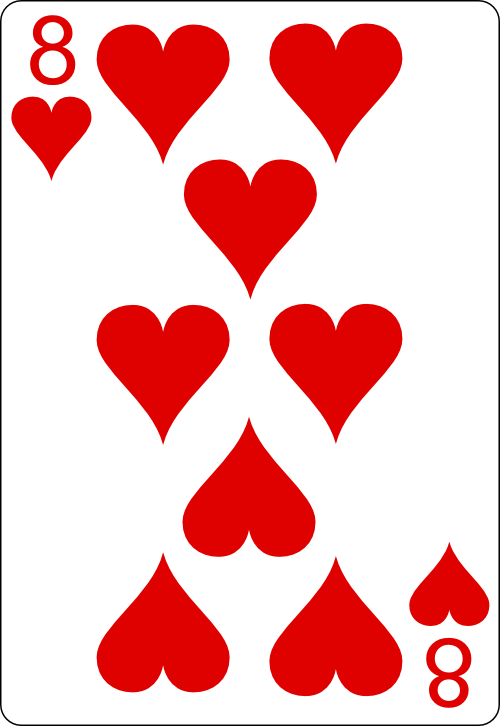
\includegraphics[height=\cardheight]{cards/8_of_hearts.png}}
\newcommand{\eightspades}{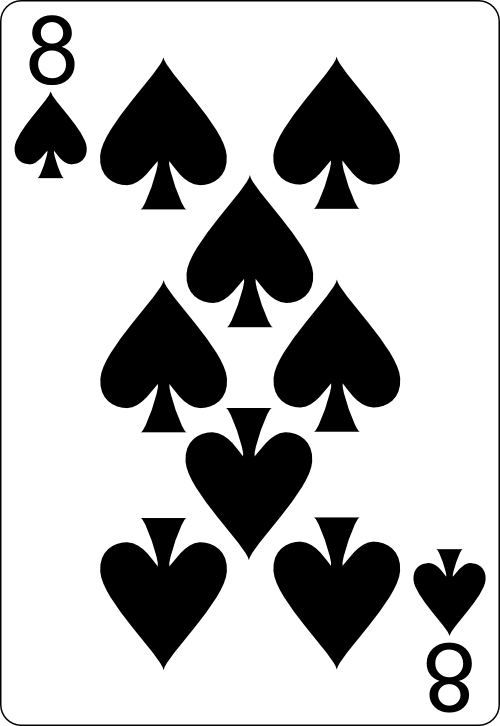
\includegraphics[height=\cardheight]{cards/8_of_spades.png}}
\newcommand{\nineclubs}{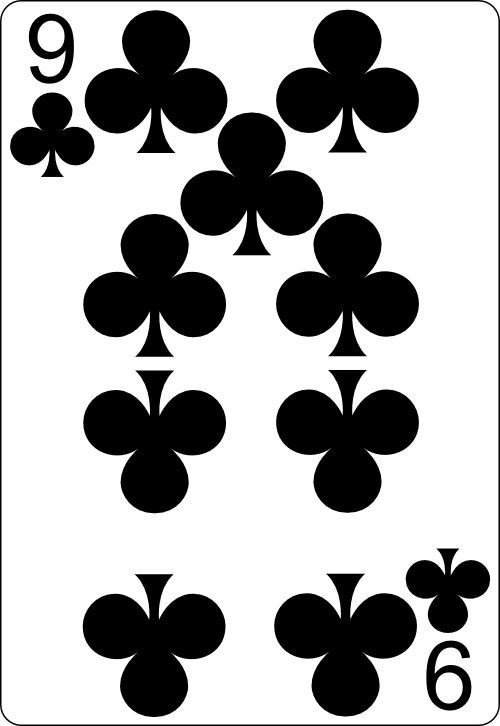
\includegraphics[height=\cardheight]{cards/9_of_clubs.png}}
\newcommand{\ninediamonds}{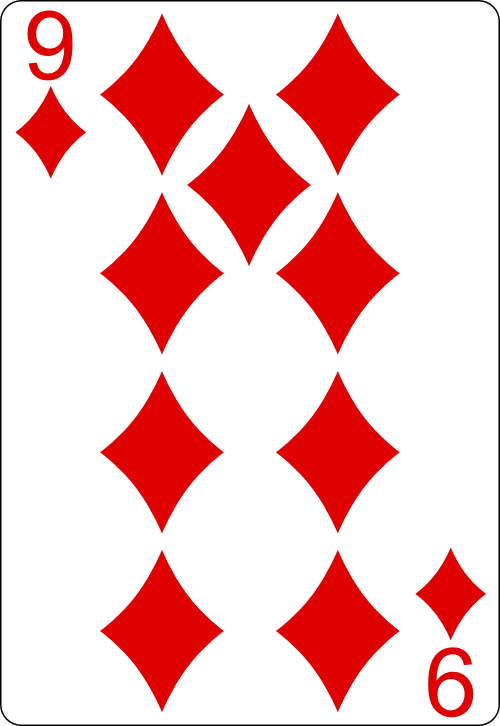
\includegraphics[height=\cardheight]{cards/9_of_diamonds.png}}
\newcommand{\ninehearts}{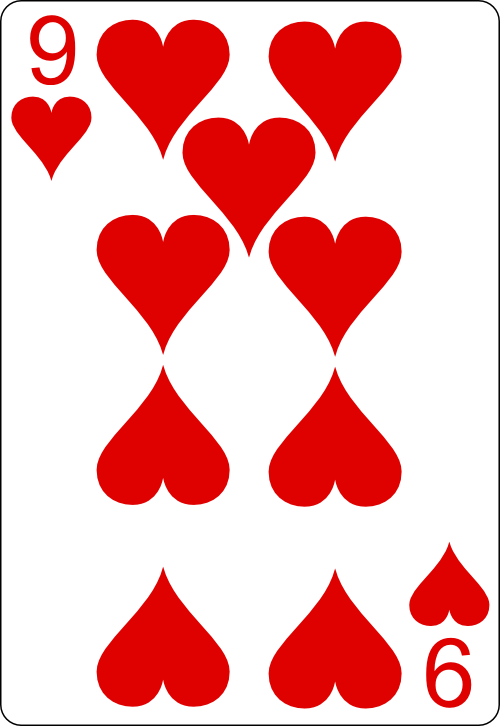
\includegraphics[height=\cardheight]{cards/9_of_hearts.png}}
\newcommand{\ninespades}{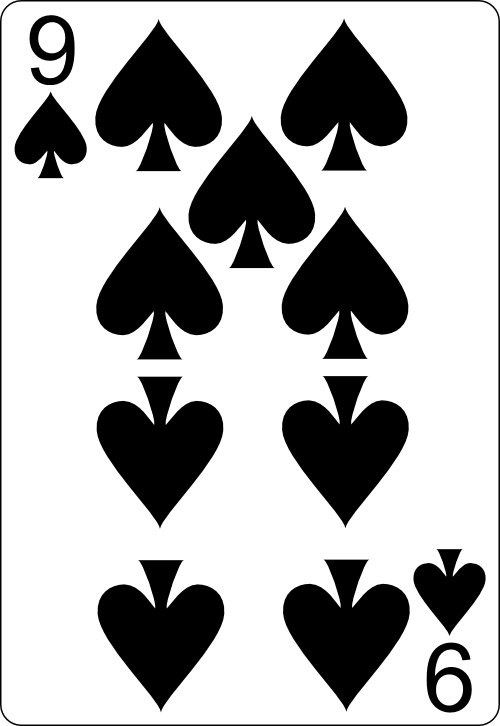
\includegraphics[height=\cardheight]{cards/9_of_spades.png}}
\newcommand{\aceclubs}{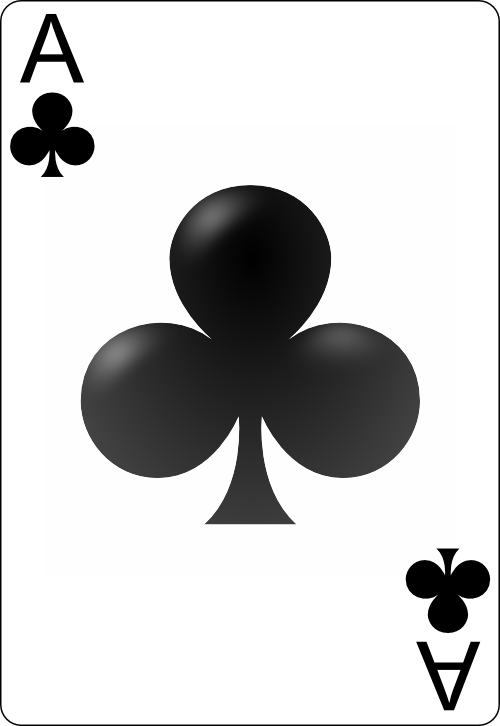
\includegraphics[height=\cardheight]{cards/ace_of_clubs.png}}
\newcommand{\acediamonds}{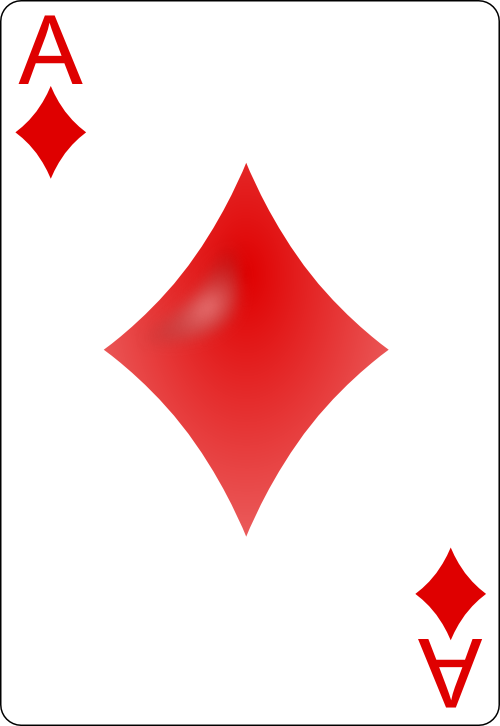
\includegraphics[height=\cardheight]{cards/ace_of_diamonds.png}}
\newcommand{\acehearts}{
\includegraphics[height=\cardheight]{cards/ace_of_hearts.png}}
\newcommand{\acespades}{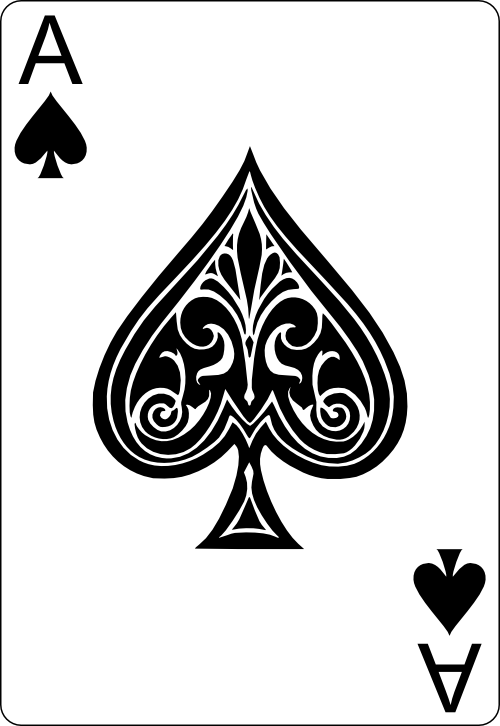
\includegraphics[height=\cardheight]{cards/ace_of_spades.png}}
\newcommand{\jackclubs}{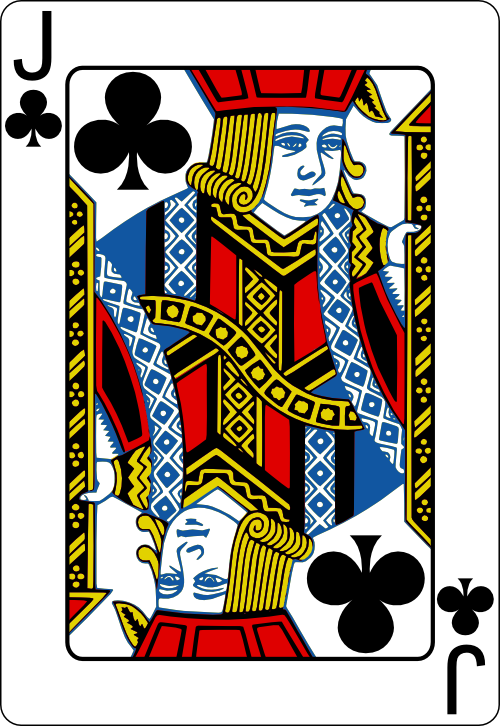
\includegraphics[height=\cardheight]{cards/jack_of_clubs.png}}
\newcommand{\jackdiamonds}{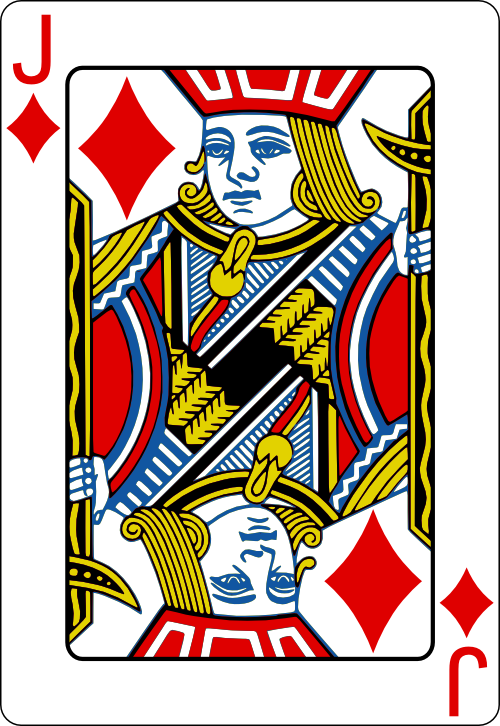
\includegraphics[height=\cardheight]{cards/jack_of_diamonds.png}}
\newcommand{\jackhearts}{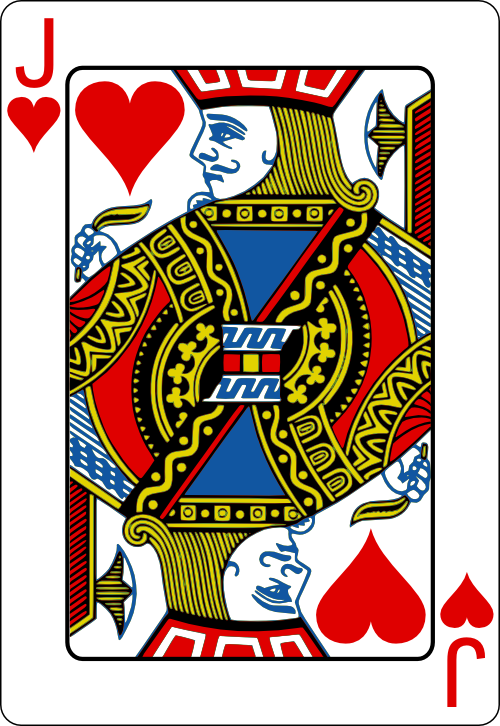
\includegraphics[height=\cardheight]{cards/jack_of_hearts.png}}
\newcommand{\jackspades}{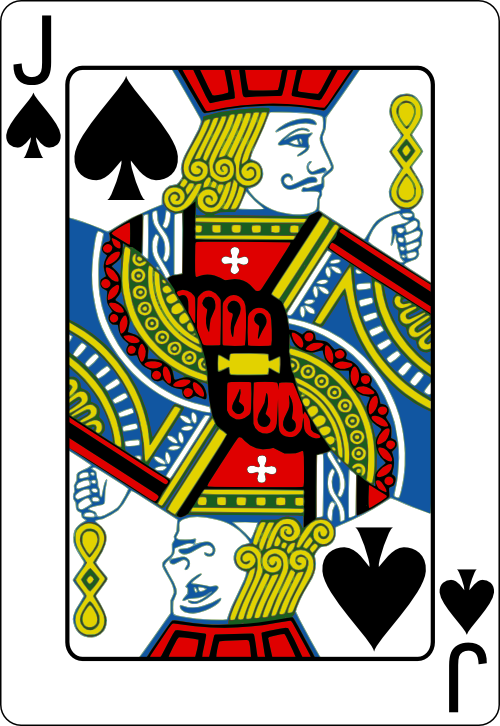
\includegraphics[height=\cardheight]{cards/jack_of_spades.png}}
\newcommand{\kingclubs}{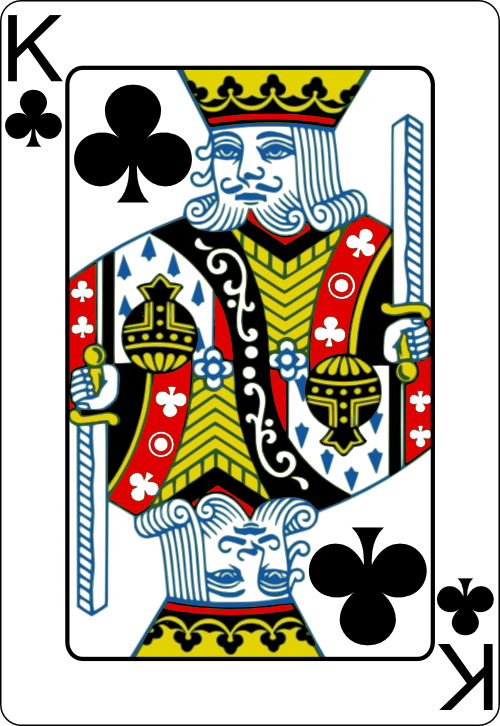
\includegraphics[height=\cardheight]{cards/king_of_clubs.png}}
\newcommand{\kingdiamonds}{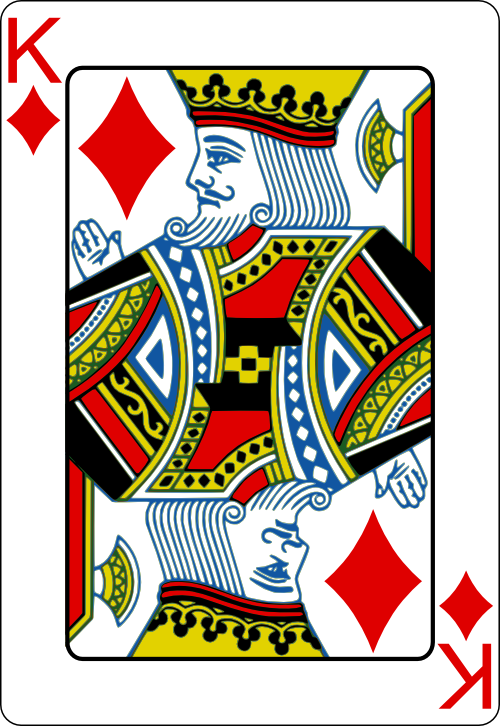
\includegraphics[height=\cardheight]{cards/king_of_diamonds.png}}
\newcommand{\kinghearts}{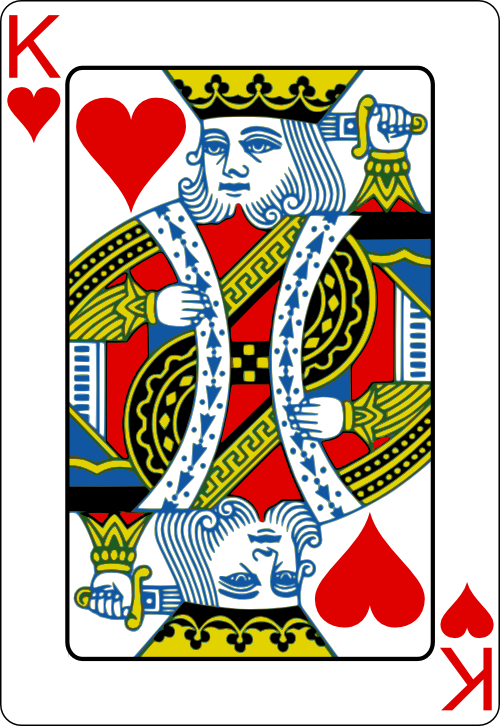
\includegraphics[height=\cardheight]{cards/king_of_hearts.png}}
\newcommand{\kingspades}{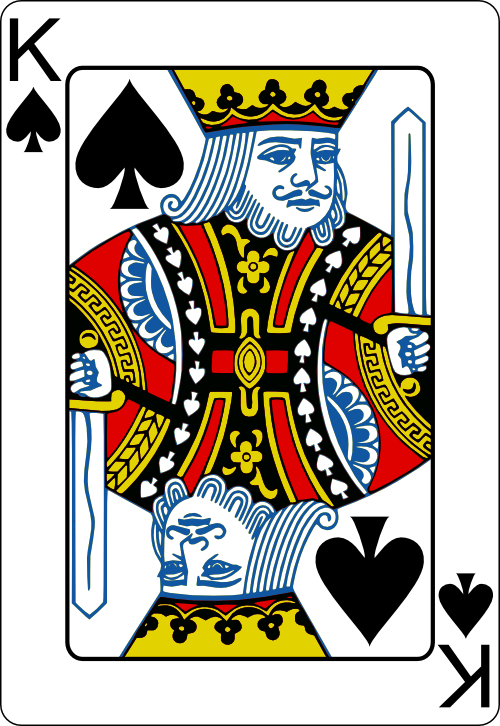
\includegraphics[height=\cardheight]{cards/king_of_spades.png}}
\newcommand{\queenclubs}{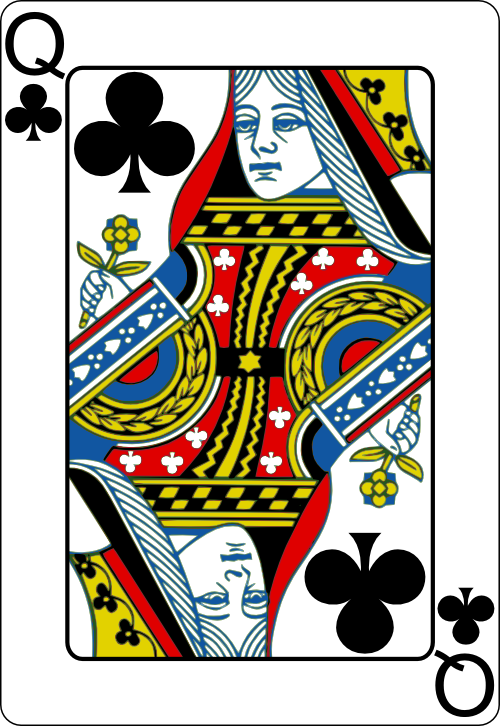
\includegraphics[height=\cardheight]{cards/queen_of_clubs.png}}
\newcommand{\queendiamonds}{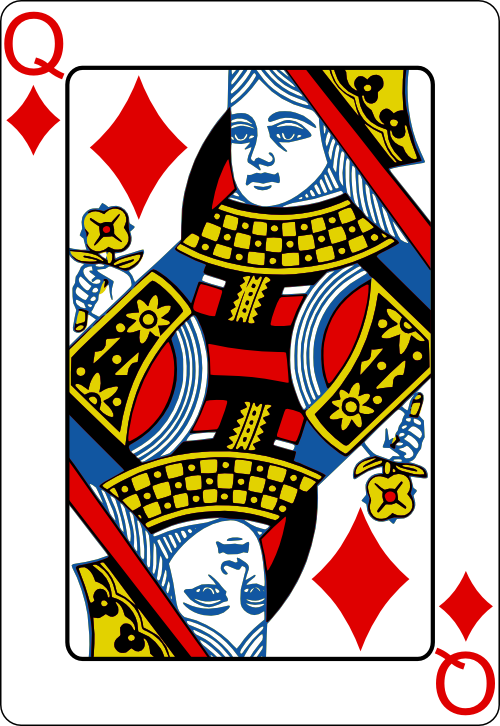
\includegraphics[height=\cardheight]{cards/queen_of_diamonds.png}}
\newcommand{\queenhearts}{\includegraphics[height=\cardheight]{cards/queen_of_hearts.png}}
\newcommand{\queenspades}{\includegraphics[height=\cardheight]{cards/queen_of_spades.png}}




\hspace{0pt}

\vfill

\begin{center}
	\includegraphics[scale=0.4]{uni_logo}
	
	\vspace{1cm}
	
	{\Large \textbf{Interim Report:} \pn \ Poker } \linebreak
	
	\begin{large}
		James Scully (4304469) \\
		psyjs20@nottingham.ac.uk \\
		G400 Computer Science \\
	\end{large}
	
\end{center}

\vfill

\begin{center}
	\textbf{Project Supervisor:} Milena Radenkovic
\end{center}

\hspace{0pt}

\pagebreak


\newcommand{\entry}[1]{
	\textbf{#1} - 
}

\newcommand{\TODO}[1]{
	\textbf{{\Large \emph{#1}}}
}



\tableofcontents



\newpage


%%%
% Page 1: 
%%%

\section{Introduction}


When one looks for a casual poker game that offers power to the actual end user, rather than attempting to fish money it can be quite difficult to find. From the authors own personal experience and observations with free and open software, it can be quite difficult to implement in some areas (such as games), however the ability to control a game how you would like and the ability to not have to rely on companies servers, trudge through in-app payments and ads is a unseen experience today. Some also do not allow for players with unreliable connections to continue; they are simply dropped from the game.  \\

I believe that many of these are far too focused on the financial aspect of the game and neglect the small groups whom simply would like another medium to play poker. This is because lobbies are often not customizable and will drop players whom do not have a good enough network connection to the lobby, so that more players are able to join.  \\

To remedy these issues, Rekop poker will be developed to handle disconnections or unstable connections by reserving their place in the lobby and the ability to join back when the player is available to. It will also not feature micro-transactions and provide the ability for players to host their own servers, with their own settings.



\section{Motivation}
Rekop poker aims to provide an alternative to other multi-player applications on the Android app store as many of these prevent user customization and introduce in-app purchases, with no ability for players to play locally on their own network. 

It is for this reason that Rekop poker is being developed, so that there is an open-source alternative where players have the control over the game. 


\section{Methodology}

Test-Driven Development has been essential so far in the development of the poker algorithm. Evaluating Texas Hold'em hands has many vectors of errors and being able to write tests before and alongside implementation helped out immensely. 

Take this snippet from the testing whether a hand is a straight or not: 

\begin{lstlisting}*[language=java]
assertTrue(new TexasEvaluator("0D 0D 2D KD AD QD JD").isStraight());
assertTrue(new TexasEvaluator("AD KD QD JD 0D QD JD").isStraight());
/* Falses */
assertFalse(new TexasEvaluator("0D 0D 0D 0D AD QD JD").isStraight());
assertFalse(new TexasEvaluator("2D 5D 9D JD 0D QD JD").isStraight());

\end{lstlisting}

This allowed me to rapidly create test cases, but more importantly easily generate cases which could break the method itself via edge cases or worst case scenarios. For example, one issue that was resolved was the method would register duplicate cards as being a straight, i.e. only 4 sequential cards would be needed. 

Agile has also been a driving methodology - primarily creating a very basic yet functional version of the software and accepting of changing requirements. For example, the backend was created first so that the gamemode itself was in an acceptable state. From here, it made it easier to visualize how the server would handle sending, receiving and processing the player's cards. 


\newpage
\section{Design}

\subsection{Overview}

The project itself is being broken down into three compartments - a backend that satisfies the core Texas Hold'em gamemode, the server which will provide the connections needed for players to play together on their own networks and the Android app, which links both of these together with the graphical interface. 

The system as a whole is very server-side, as this holds all the data instead of the clients. Appendix entry 3 shows the basic design of the system, whereby the client only receives its current hand, the ranking of their hand and the cards currently shown on the table. 

\subsection{Backend}

The backend is written solely in Java as the language itself is platform agnostic - Android being reliant upon Java (bytecode). It has been broken down in such a way that game modes other than Texas Hold'em can be added to it, enabling further development down the line. 

For example, we've created data classes for Faces and Suits, each containing values for easy comparison. Furthermore, we've created a Deck class that allows for the user to pull a random card from a standard 52-card deck and ensure that it hasn't been pulled before. These building blocks allow for future development by providing the basics needed in a standard card game.



\subsection{Server}

Initially, an idea as defined in our Vision and Scope document was to use a UPnP / Peer to Peer approach, however this is infeasible as a key requirement of this project is disconnection-tolerance. This is because if the host is to lose connection permanently or temporarily, the rest would be unable to play.
This is where we've opted for a client-server approach; as this allows atleast for one solid host, separate from the clients whom are likely to suffer connection issues. 

The servers design is such that on the start of the game, the server knows exactly what cards are going to be placed on the actual table, i.e. the initial flop (3 cards), turn and river albeit these will not be released to the player until necessary. It is responsible to send what cards each player has, and will utilize the previously mentioned Deck object to deal hands out. 

Therefore, the only messages required by the client to send are their actions, such as how much they are betting, whether they fold or raise. 

\begin{center}
\includegraphics[scale=0.65]{server_diag}
\end{center}

\newpage
\subsection{User Interface / Android application}

The most critical part and the binding element of this project is the actual mobile application itself. The user interface is to be kept simple, with the main menu being a simple strip of buttons that can be added to for extra gamemodes or features. There is a navigation bar that will allow the user to switch between playing, statistics, profile and to exit. 
The interface is required to be simple, as this allows for intuitive and good user experience with the application. \\

The following figure shows how we've changed our initial wireframe slightly. As we've implemented it into Android, we've attempted to make it appeal to certain conventions, such as using the Hamburger icon for the menu and moving it to the side of the screen.

\begin{figure}[h]
	\makebox[\textwidth][c]{
	\begin{subfigure}[h]{0.5\textwidth}
		\includegraphics[width=\textwidth]{menuwireframe}
		\caption{Wireframe}
	\end{subfigure}	
	~
	\begin{subfigure}[h]{0.6\textwidth}
		\includegraphics[width=\textwidth]{menuapp}
		\caption{Prototype}
	\end{subfigure}	
	}
	
	\caption{A slightly altered production of wireframe}
	
\end{figure}

\subsection{User Interface / Android application}

The most critical part and the binding element of this project is the actual mobile application itself. The user interface is to be kept simple, with the main menu being a simple strip of buttons that can be added to for extra gamemodes or features. There is a navigation bar that will allow the user to switch between playing, statistics, profile and to exit. 
The interface is required to be simple, as this allows for intuitive and good user experience with the application.









\subsection{Algorithms}

\entry{Hand Strength}
The algorithm for hand-strength is very basic and as such is ineffcient, however this is not the main focus of the project. The base of our algorithm is in a TexasEvaluator class, whereby we test each potential result i.e. straight, flush in their own methods. We then sequentially run these methods in order of ranking, so that we can return a result. 


\entry{Win evaluation}
Win evaluation can be done by sorting each players hand by result, i.e. Royal Flush, Four of Kind, Straight. If each player has a unique result, then we can simply take the top result, in this case Royal Flush. If two players contest the highest result, e.g. a Straight, then we'll look at the highest card in the TResult object, which determines each players result and the highest card. 

If two players contest the highest result, but have the same highest card, then the pot is split as is the normal result in poker. 


\section{Implementation}

\subsection{Project Requirements}
Our requirements for the project were not particularly specific, however some core ones were defined in our vision and scope, aswell as project proposal. 

\subsection{Backend}
\textbf{Functional}
\begin{itemize}
	\item Programmed in Java (or Kotlin)
	\item Able to generate a result (i.e. 3 of kind) from the players hand and table
	\item Abstracts elements of card-based games (i.e. hands, cards, faces)
\end{itemize}
%\textbf{Non-Functional}
%\begin{itemize}
%	
%\end{itemize}

\subsection{Server}
\textbf{Functional}
\begin{itemize}
	\item Runs on Linux and Windows
	\item Handles the evaluation of games internally
\end{itemize}

%\textbf{Non-Functional}
%\begin{itemize}
%
%\end{itemize}

\subsection{Application}

\textbf{Functional}
\begin{itemize}
	\item Runs on devices using Android KitKat
	\item Allows for connecting to servers via IP address
\end{itemize}
\textbf{Non-Functional}

\begin{itemize}
	\item Presents a simple, uncluttered interface
	\item Presents a server browser for online matches
\end{itemize}

\newpage


\subsection{Card class}
As mentioned previously, we wanted to add base classes for the ability to add other card games later on. As most card games utilize the standard 52-card deck, we created the Card class to hold typical data - the Face of the card (e.g. Queen) and the Suit (e.g. Clubs). \\


\subsection{Face}
For the face class, we opted to use an enum as these are generic datatypes that are both easy to read in code (they do not need to necessarily be initialized) and can be assigned a value similar to normal classes. 

This was chosen because it simplifies reading the code, but they can also easily define other values in their constructor. The code below shows this, as we can set a custom display value, e.g. "Three" and a value for the card. Later on, we can use these values to sort hands and make determining straights much easier.

\begin{lstlisting}*[language=java]
public enum Face {

	// these can be accessed as Face.TWO, Face.ACE, etc. 
    TWO   ("Two", 0),
    THREE ("Three", 1),
    FOUR  ("Four", 2),
    FIVE  ("Five", 3),
    SIX   ("Six", 4),
    SEVEN ("Seven", 5),
    EIGHT ("Eight", 6),
    NINE  ("Nine", 7),
    TEN   ("Ten", 8),
    JACK  ("Jack", 9),
    QUEEN ("Queen", 10),
    KING  ("King", 11),
    ACE   ("Ace", 12);

    private final int val;
    private final String str;

    Face(String display, int value) {
        this.str = display;
        this.val = value;
    }
}
\end{lstlisting}

\newpage
\subsection{Evaluating Hands of Texas Hold'em}

I decided it was best to have multiple methods for evaluating a hands rank as other methods of implementing this involved lookup tables or other more convoluted methods, such as representing cards as 52-bit numbers and performing bitwise operations on them. Though lookup tables are very quick to evaluate \cite{lookup}, I felt that for this project having clear code was more suitable as we intend to open-source it, the same applies with bitwise operations. 

The evaluate method itself contains the following code: 

\begin{lstlisting}*[language=java]
    public TResult evaluate() {
        // these conditions must be done in sequence, for order of rankings
        TResult kindOutput = getKinds();
        // this is required so that StraightFlushFlag is set
        TResult isStraight = isStraight();
        // variable to hold each test
        TResult result = null;
        // assignment in if statement is to remove calling method twice
        if( (result = isRoyalFlush()) != null)
            return result;
        if(StraightFlushFlag)
            return isStraight;
        // because kindOutput may be null, we need to ignore it to get past to straight
        try {
            if(kindOutput.rank == Rank.FOUR_OF_KIND)
                return kindOutput;
            if(kindOutput.rank == Rank.FULL_HOUSE)
                return kindOutput;
        } catch (NullPointerException ignored) { }
        if( (result = isFlush()) != null)
            return result;
        if(isStraight != null)
            return isStraight;
        if(kindOutput != null)
            return kindOutput;
        // the highest card will always be first as we use a sorted collection
        return new TResult(cards.get(0).face, Rank.HIGH_CARD);
    }
\end{lstlisting}


\newpage
\subsection{Determining a Straight}
Determining whether a hand is a straight would be difficult had we not assigned values to the Face values of our cards. Take the following table, whereby the first two cards are the players, the other 5 are on the table. \\

\begin{center}
\tendiamonds \twoclubs \ \ \ \ \ \ \  \eightclubs \ninehearts \sixdiamonds \fiveclubs \sevenspades
\end{center}

This hand's highest rank would be a straight, as we 10 - 5 in the hand; though they are not displayed as in order. \\

Take for example we start off with the first card, 10 of Diamonds. We would have to find any card on the table that is either a Jack or a 9. From here, we would then have to branch off and see if there is a card that is a Queen or an Eight, for either direction. This would have to be done for each card on the table, and optimizations would make the code more complex and introduce more areas where bugs or incorrect results can slip in.\\

However, since we have assigned each of the Faces values as seen previously in Section 5.2 we can use Java's Collections library to sort our cards from highest to lowest. This way, we only need to search in one direction, i.e. if the next card is lower than our current one; which is shown in Appendix entry 4.


\newpage
\section{Progress}
\subsection{Management}


To help me manage what needs to be done in the project and primarily drive development, GitLab issues tracker have been made for various tasks that need to be completed. These are easy to read via the use of labels and offer reminders through school email. In addition to this, branches are created for each issue to manage changes to code.  \\

In the initial design stages, I focused on the vision and scope whereby outlining the ideal product but also the bare essentials for the project. Working under agile principles, I focused on getting a usable algorithm for evaluating poker hands as this gives us early ideas from where to go next or problems that would arise; once we had this to a good state, research for how the server will handle sending these objects or communicating became easier.  \\

Appendix entries 1 and 2 show the old and the new Gantt charts. Upon developing the backend, I realised that no databases and thus database classes were needed in this part. Later on during the end stages of the servers development, databases will be used for online play, and can be removed at this stage. Therefore, server tasks aswell as implementing them into the Android app have been brought forward, as these are critical.  \\

\subsection{Contributions and Reflections}

A key goal of all software is that it must be efficient - both in terms of code complexity and performance. Upon undertaking this project it was naively assumed that, given how easy it is to recognize the outcome of a poker round in reality, it wouldn't be too difficult to implement efficiently through code. \\

It is therefore that the algorithm currently used is very compartmentalized, and potentially slower than some implementations (such as look-up tables or doing bit-wise operations). For example, it takes between 50 - 100ms for one result to be calculated on a desktop computer. Since most servers will be running on one, it doesn't particularly matter about the performance as much as the other aspects of the program.\\

Reflecting upon how I assumed Test-Driven Development would take much of our time before and during up and that we did not have "too much time to write tests and develop a fully-functional program", this couldn't have been further from the truth. Having instant feedback on whether it passed, what the result was and the ability to debug into it was essential. \\

Although, initially I was under the assumption that each test case was going to have to be made up of newly created objects. Test cases wrote this way were taking too long and becoming a nuisance to write. Instead, I created a factory-esque pattern within the evaluator class itself to resolve, for example, "0D 0D 2D KD AD QD JD" into an actual hand + table cards.  \\

The example below shows how writing test cases becomes much easier through this method, rather than creating a new object for each test case.

\begin{minipage}{.5\textwidth}

\begin{lstlisting}
TexasHand FLUSH_FOK = new TexasHand(
    new Card(Suit.CLUBS, Face.FOUR),
    new Card(Suit.CLUBS, Face.FOUR),
    new Card(Suit.CLUBS, Face.FOUR),
    new Card(Suit.CLUBS, Face.FOUR),
    new Card(Suit.CLUBS, Face.ACE)
);
...
public void isFlush() {
    assertTrue(FLUSH_FOK.isFlush());
\end{lstlisting}
\end{minipage}
\begin{minipage}{.5\textwidth}

\begin{lstlisting}[breaklines=true]
assertTrue(new TexasEvaluator("4C 4C 4C 4C AC QS JC").isFlush());
\end{lstlisting}
\end{minipage} \\

\subsection*{Conclusion}

Currently, I am satisfied with the backend of the project as the main area of concern was accuracy in determining the outcome of a game. The use of unit tests has taught me how to effectively break a problem down into small, testable blocks of code and then re-construct them into an algorithm. \\


However, I think that one area to work on would be time management and consequently gauging how much time tasks will take; in particular the next step which is the server. This next step is not so easy to debug as it is not as easy as sequencing certain blocks of code together to create a system and most certainly not easy to debug. Therefore, I have pushed these tasks to the front of jobs to be done and allowed myself more time for these.

\newpage

\section{Appendix}

\textbf{1. Old Gantt Chart} \\

\includegraphics[width=\textwidth]{gantt_chart}

\newpage
\textbf{2. New Gantt Chart}

Color chart:

Purple = completed \\
Green  = to be completed\\
Orange = moved forward\\
Red = deleted\\

\includegraphics[width=\textwidth]{modified_gantt}


\newpage
\textbf{3. Whole system design}

\includegraphics[width=\textwidth]{wholesystem}


\newpage 

\textbf{4. Straight method}

All cards are sorted before this and other methods in the evaluator are called.

\begin{lstlisting}
    public TResult isStraight() {
        int valStreak = 0;
        int suitStreak = 0;
        int origin = 0;

        // our previous value going in should be the first in the sorted array
        // note: cards is a class member containing all cards in the evaluator, 
        // sorted high to low.
        int previousVal = cards.get(0).getValue();
        Suit previousSuit   = cards.get(0).getSuit();

        for(int i = 1; i < 7; i++)  {

            // these are the attributes of card i
            Card card   = cards.get(i);
            Suit suit   = card.getSuit();
            int  value  = card.getValue();

            // if we have a previous card of same value, just skip over.
            if(previousVal == value)
                continue;

            // if the previous card was higher than the current, then add to streak
            // else, reset counter to 0.
            if(previousVal == value + 1) {
                valStreak++;

                if(suit == previousSuit)
                    suitStreak++;
                else
                    suitStreak = 0;

            } else {
                valStreak = 0;
                origin = i;
            }

            // if we've already managed a straight, then return true.
            // note that this should return the highest STRAIGHT, as we're descending down.
            if(valStreak == 4) {
                // this removes the need for ANOTHER function for Strt. Flushes.
                if(suitStreak == 4)
                    StraightFlushFlag = true;

                Face high = cards.get(origin).face;
                Rank result = StraightFlushFlag ? Rank.STRAIGHT_FLUSH : Rank.STRAIGHT;

                System.out.println("Returning true, high card: " + high + "rank:" + result);

                return new TResult(high, result);
            }

            previousVal = value;
            previousSuit = suit;
        }
        return null;
    }
\end{lstlisting}




\newpage
\section{Bibliography}

\renewcommand\refname{Bibliography}
\begin{thebibliography}{9}

\bibitem{lookup}
\begin{flushleft}
	Luís Filipe Teófilo, Luís Paulo Reis, Henrique Lopes Cardoso \\
	\textit{Speeding-Up Poker Game Abstraction Computation: Average Rank Strength} \\
	Source in paragraph: \textit{2. Background} \\
	Retrieved from \url{https://www.aaai.org/ocs/index.php/WS/AAAIW13/paper/view/7083/6489}
\end{flushleft}


\end{thebibliography}


\end{document}